%\usepackage{here}
%\usepackage[dvipdfmx]{graphicx}
%\usepackage{amsmath,amssymb}
%\usepackage{array,booktabs} %表のためのarray環境

%\begin{document}
\section{NaIで取得したデータの解析と結果・考察}
主に測定した信号から欲しい情報を取り出すための解析に関する部分と得られた情報から実際の測定した量を解析する部分にわけられる.特に前半の信号解析ではパイルアップ信号を取り除く処理を行い,情報を取り出す解析を行った.後半については寿命と$g$因子の測定という時間に関する値を用いる解析では通常のFittingを行った.一方,ミッシェルパラメータでは時間情報に基づいてスピンの情報を得ると共に,エネルギー情報に対し測定器の電磁シャワーの応答に基づくFittingを行った.

\subsection{信号解析}
主にNaI検出器で測定した波形解析の手法について述べる.実際に測定データの中で典型的なものの一つを\figref{hatano_fig:rawdata}に示す.波形解析ではここからFinger Counter(チャンネル1)が鳴っている時にNaIに落とされたエネルギーと鳴った時の時間という2つの情報を抽出した.この際に高周波のノイズが小さくないという事とNaIの減衰時間が長いという事の2つが解析時の注意点となった.特に前者は信号から鳴ったという判定をするためにピーク検出をする際に誤った判定を行う可能性があった.それは本来は1回の信号であるのにノイズがのることにより短い時間に何度も振動する影響で複数のピークとして誤認識してしまう危険性があった.そのため,今回の解析ではノイズ除去の処理を最初に行った.その後ピーク検出を行った後に時間情報とエネルギー情報を取り出すが,この際に後者の注意点の影響があった.実際に\figref{hatano_fig:rawdata}でも分かるように別の由来のNaI信号が重なり合う(パイルアップ)現象を起こしている.これを処理しないままで適当な領域で積分を行ってもエネルギーを求めると,本来の信号でないものの影響でエネルギーが大きく見積もられる原因となる.このため,今回の解析では波形データのサンプリングを行いそれに基づきパイルアップしてない部分の波形からパイルアップしている部分に外挿し,その分の補正を行った.以下具体的な処理について述べる.
\begin{figure}[bht]
  \centering
  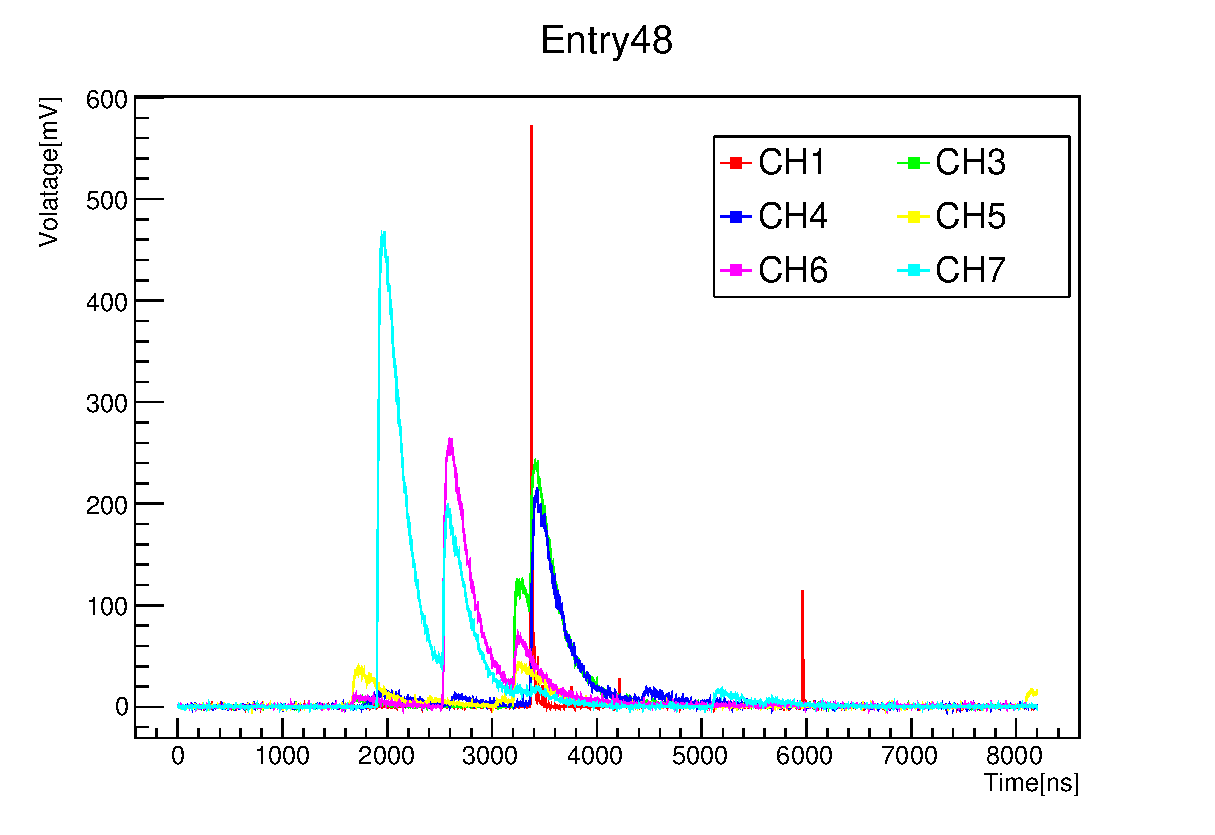
\includegraphics[width=0.8\textwidth]{figure/hatano/rawdata.eps}
  \caption{NaI検出器の測定信号}
  \label{hatano_fig:rawdata}
\end{figure}

\subsubsection{ノイズ除去}
ピーク検出の際に邪魔となる高周波でのっているノイズを除去することについて考える.今回はピーク検出の前段としての概ね高周波成分が処理されてピークと誤認識するような大きな変動がなくなればいいので,簡単に実装ができかつ高速に処理できるという観点で単純移動平均をとるということを行った.具体的には各サンプリング点で前後4サンプリング,計9サンプリングの平均をとった.実際にノイズ除去を行った前後の信号の差異は\figref{hatano_fig:smoothdata}(\figref{hatano_fig:smoothdata}と同じデータの一部)のようになる.薄い色で示したのが元の信号で濃い色で示したのがノイズ除去を行った信号である.CH6の左側の信号などはノイズによって2つのピークのように見かけ上分裂していたのが改善しているのが分かる.

\begin{figure}[bht]
  \centering
  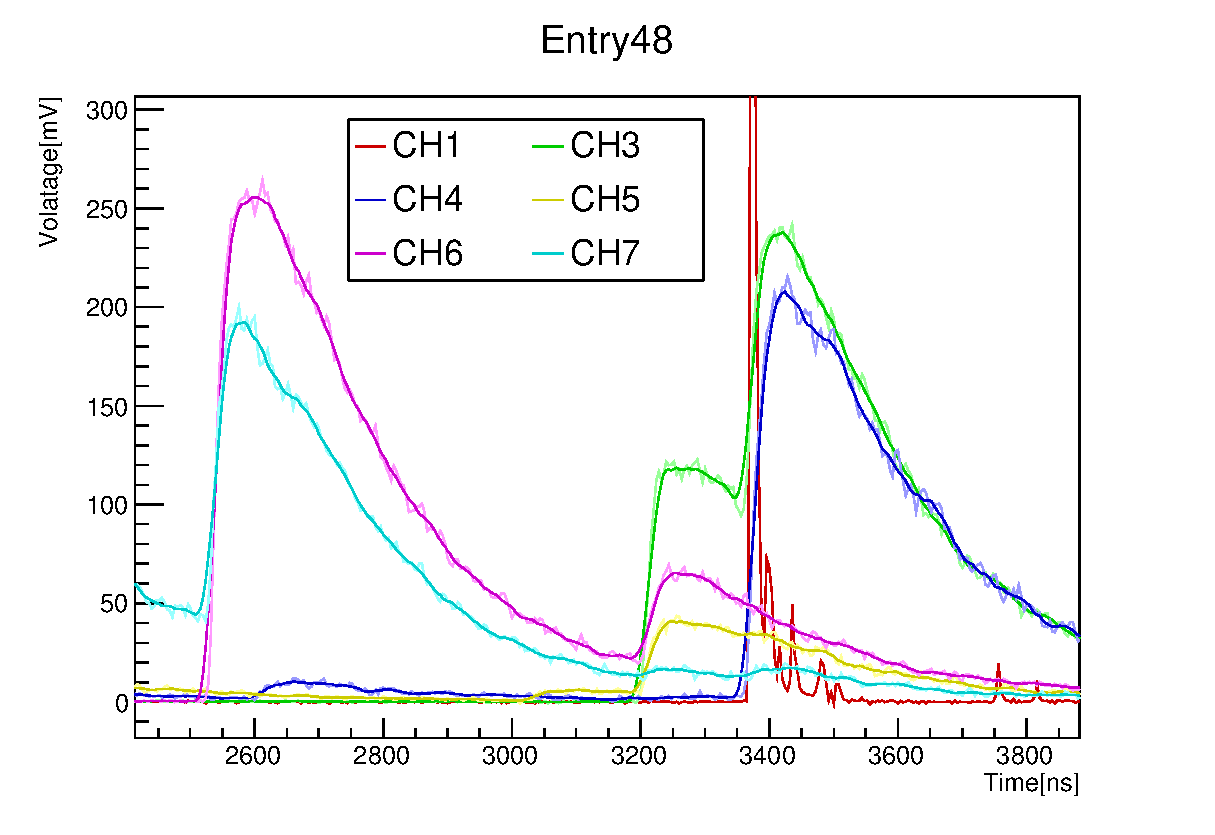
\includegraphics[width=0.8\textwidth]{figure/hatano/smoothdata.eps}
  \caption{ノイズ除去された測定信号}
  \label{hatano_fig:smoothdata}
\end{figure}

\subsubsection{ピーク検出}
以上のノイズ除去を行った信号を元にピーク検出を行うことを考える.基本的にはしきい値を適切に設定しそれを超えたところからピークが始まったと考えることにする.ただし,この方法ではパイルアップしてる際には過剰に信号を検出しうる事がありうる.すなわち,本来の適切な信号の前にあるパイルアップの原因となった信号によりオフセットがのることになり,パイルアップしている際のみその分しきい値が下がってるのと同じ状態になり低エネルギーのものを拾いやすくなる.そのため,しきい値のベースラインとなる値を信号が来る前のピークが無い部分における最小値とすることにした.このような工夫をすることで,パイルアップしてる際はベースラインが高くなるため,パイルアップによるオフセットの影響をある程度キャンセルすることができる.そのようにしてピーク検出を行った際の信号が\figref{hatano_fig:peakdata}である.それぞれ色が濃くなっている部分がピークとして判定されている領域で,点で示されているのがピーク(最大値)である.

\begin{figure}[bht]
  \centering
  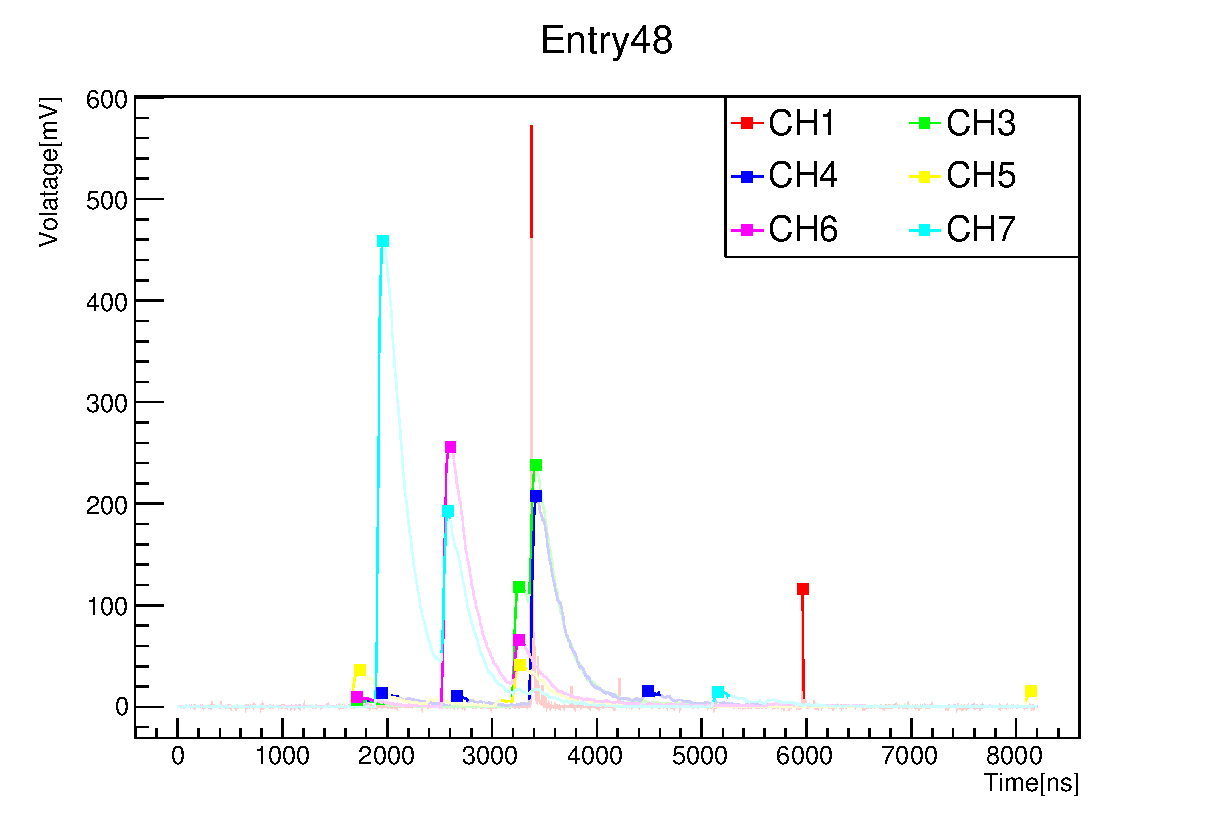
\includegraphics[width=0.8\textwidth]{figure/hatano/peakdata.eps}
  \caption{ピークとして検出された信号}
  \label{hatano_fig:peakdata}
\end{figure}

\subsubsection{波形データの抽出}
パイルアップに対処するために全イベントからパイルアップしていない時の波形データを抽出しそれにより外挿を行うことを考える.今回は主にNaIは減衰時間が長くその部分でパイルアップが起きていると考えた.すなわち,ピークの部分は全て検出できているとし立ち下がる部分によるパイルアップのみに対処した.具体的には波形データのサンプルから減衰時間を測定し,それを元にピークから立ち下がり部分に外挿$\exp(-t/\tau)$($\tau$:減衰時間)をするというアプローチをした.
ピーク検出された信号のうちパイルアップしていない信号の減衰部分に対して指数関数でFittingを行った.具体的にパイルアップしていない信号とは,次のピーク信号がくるまで400ns以上の間隔があるものとした.また減衰部分の領域はピーク部分の影響やバックグラウンド部分の影響を減らすため,ピークの時間から80ns後から次の信号が来るまでの最後の10\%を外した領域とした.これに対しFittingを行いFittingの$\chi^2$のConfidenceLevel(CL)が50\%を切るものはFittingが失敗ないしは適切な信号ではなかったと考え捨てた.実際のFittingを行った時の様子が\figref{hatano_fig:decayfit}である.濃い色で示されているのがFittingした関数である.赤の線で示したのはCLが50\%以下であったため捨てたFittingである.

\begin{figure}[bht]
  \centering
  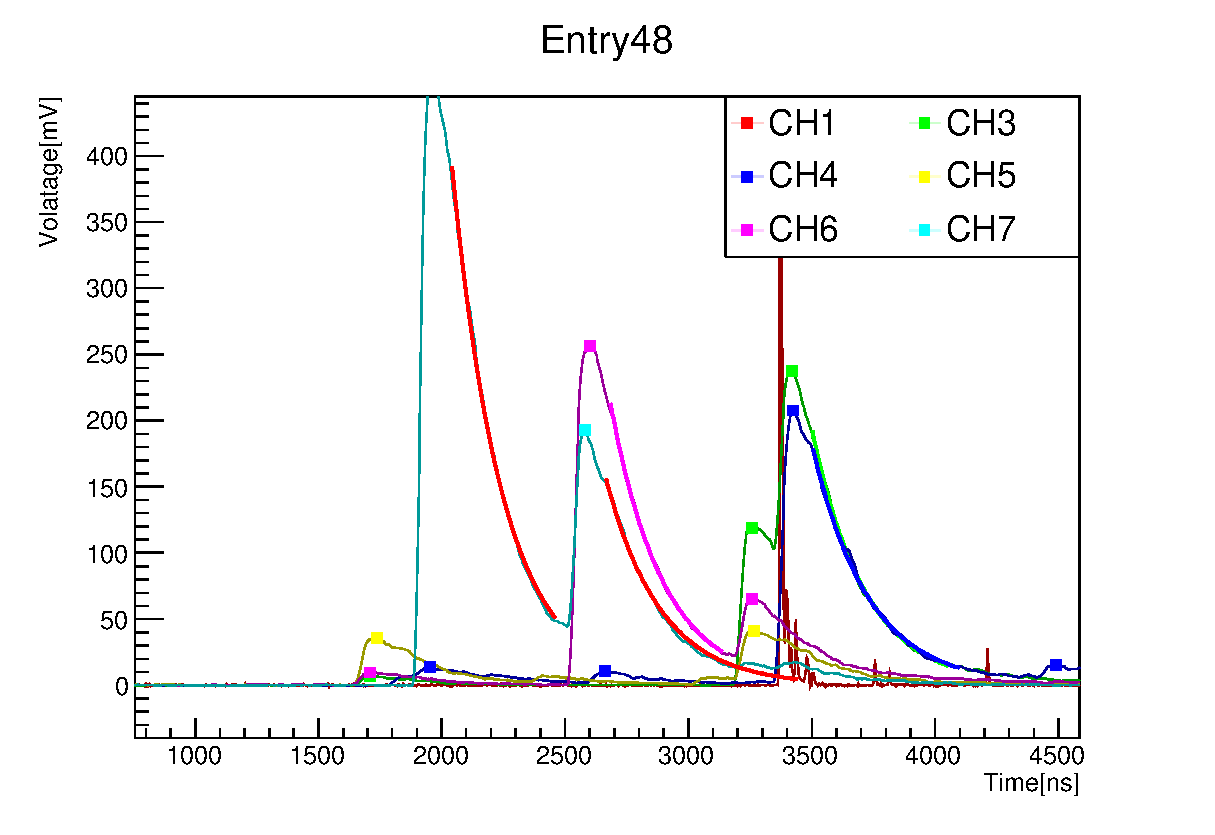
\includegraphics[width=0.8\textwidth]{figure/hatano/decayfit.eps}
  \caption{波形データにたいするFitting}
  \label{hatano_fig:decayfit}
\end{figure}

これを全ての測定データに行い出された結果が\figref{hatano_fig:decaytime}である.チャンネル7のヒストグラムは2峰になっているが,これは2つのNaIの信号をアナログ的に加算したため異なる減衰特性のNaIの信号がひとつにまとめられたことに由来すると考えられる.実際他のチャンネルのデータのピーク値もその程度のばらつきがある事が確認される.また外挿の際にはピークからそれがどちらの信号であるかを識別する事はできないため,これらを選別することを考えず各チャンネル毎に減衰時間を単純に平均し,それを減衰時間とした.
\begin{figure}[bht]
  \centering
  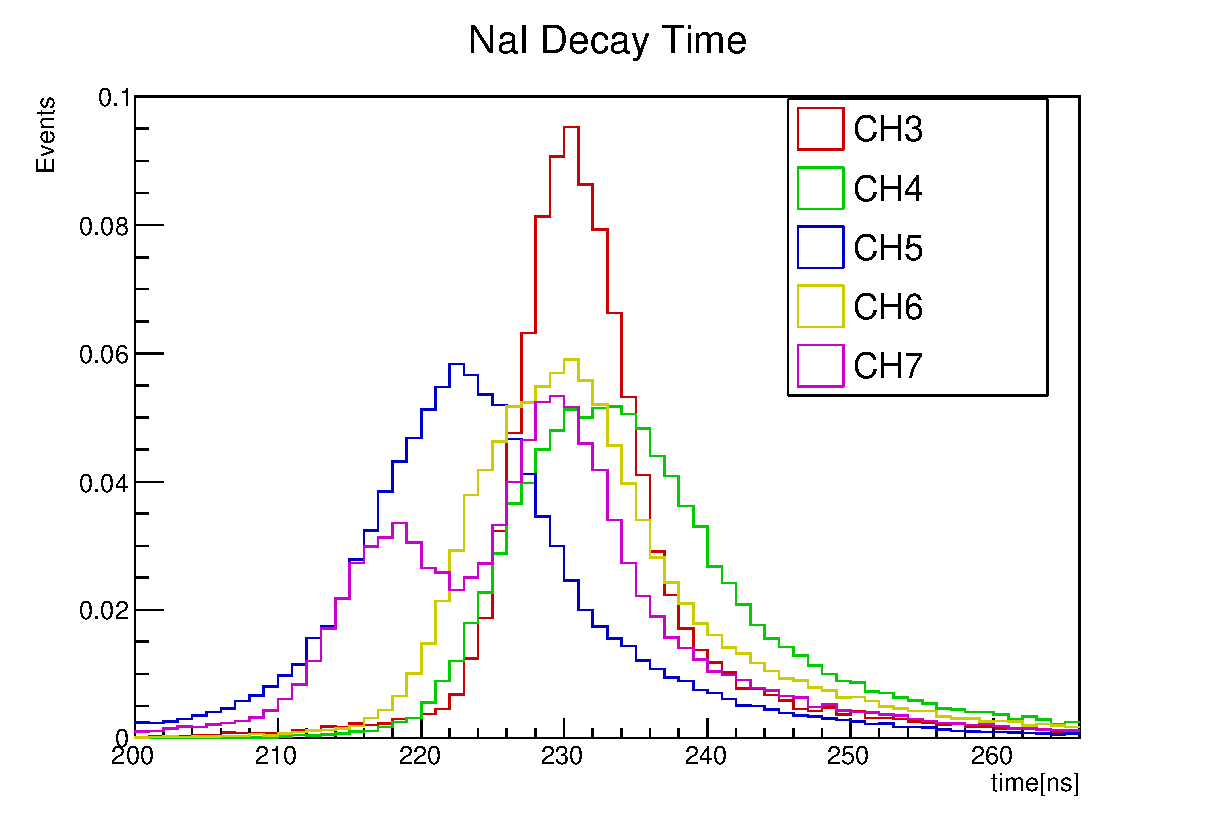
\includegraphics[width=0.8\textwidth]{figure/hatano/decaytime.eps}
  \caption{NaIの減衰時間の測定}
  \label{hatano_fig:decaytime}
\end{figure}

その結果が\tabref{hatano_tab:decaytime}である.

\begin{table}[bht]
  \centering
  \caption{各チャンネルにおける減衰時間}
  \begin{tabular}{cc}\\ \hline
    チャンネル番号 & 減衰時間(ns) \\ \hline
    3 & 232.6 \\
    4 & 236.7 \\
    5 & 224.2 \\
    6 & 233.4 \\
    7 & 228.6 \\ \hline
  \end{tabular}
  \label{hatano_tab:decaytime}
\end{table}

\subsubsection{波形データの外挿}
波形データの外挿は次のように行った.ピークが終わった後の減衰中に次のピークが見つかった場合は,減衰時間中の最小値から前5サンプリング分のデータを基準に求めた減衰時間(\tabref{hatano_tab:decaytime})の指数関数を外挿した.実際に外挿を行った時の信号の様子が\figref{hatano_fig:analysis}である.濃い色の線で示しているのが外挿した波形データである.

\begin{figure}[bht]
  \centering
  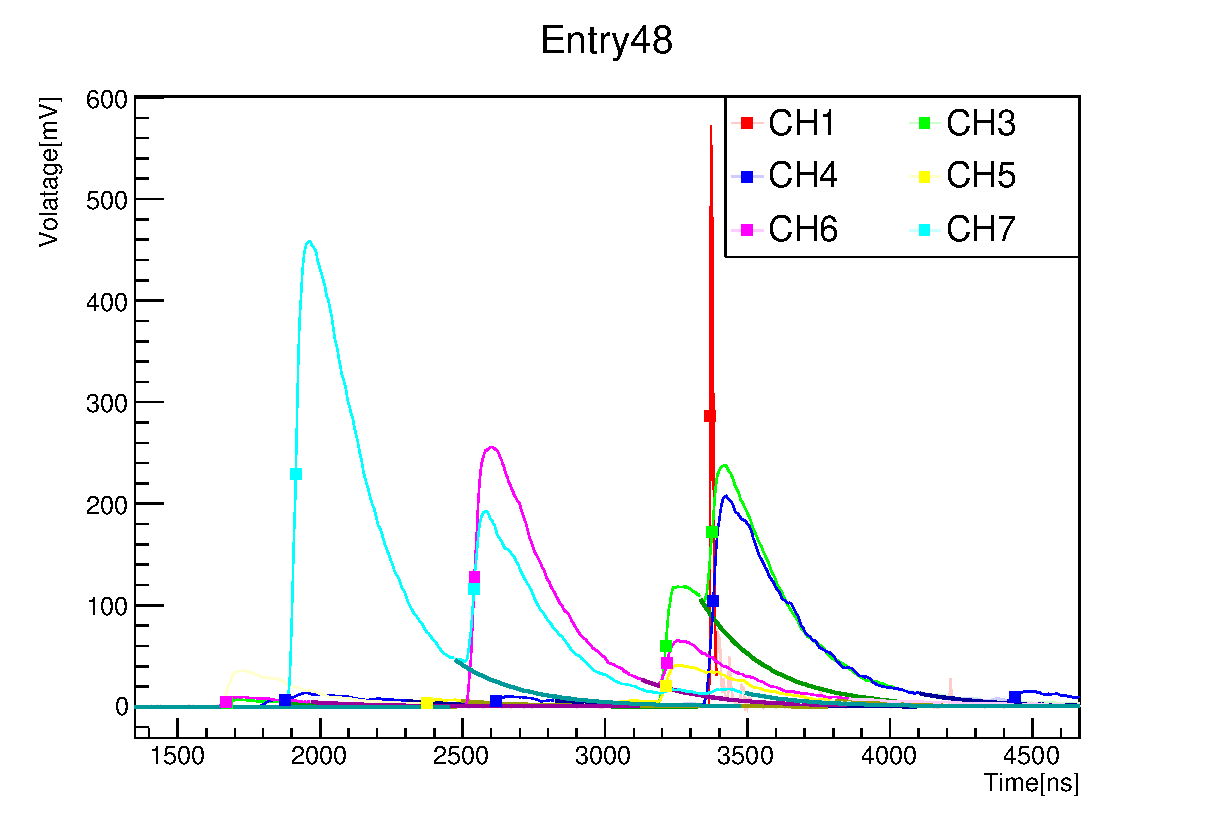
\includegraphics[width=0.8\textwidth]{figure/hatano/analysis.eps}
  \caption{波形の外挿の様子}
  \label{hatano_fig:analysis}
\end{figure}

\subsubsection{解析データの抽出}
以上の解析で主に各チャンネルごとに信号から情報を抽出できる準備ができたので,これを元にピークの50\%の値を超えたところを時間として,前のピークから外挿された分を差し引き,自らの外挿分を加えた積分値をエネルギー抽出とした.

さらに本当に欲しいデータは標的から飛んできた陽電子の信号は手前のフィンガーカウンタを通ったデータだけであるので,フィンガーカウンターの信号と同時に鳴ったとみなせるNaI信号を考えたい.シンチレータの差などからわずかに時間の基準からずれている分を考慮するため,フィンガーカウンターと各NaI信号の時間差をとると\figref{hatano_fig:coincidence}となった.よって,フィンガーカウンターが鳴った時を基準にその後20(ns)の間に鳴ったNaI信号のエネルギーの合計値をフィンガーカウンターが鳴った時に入ったエネルギーとした.

\begin{figure}[bht]
  \centering
  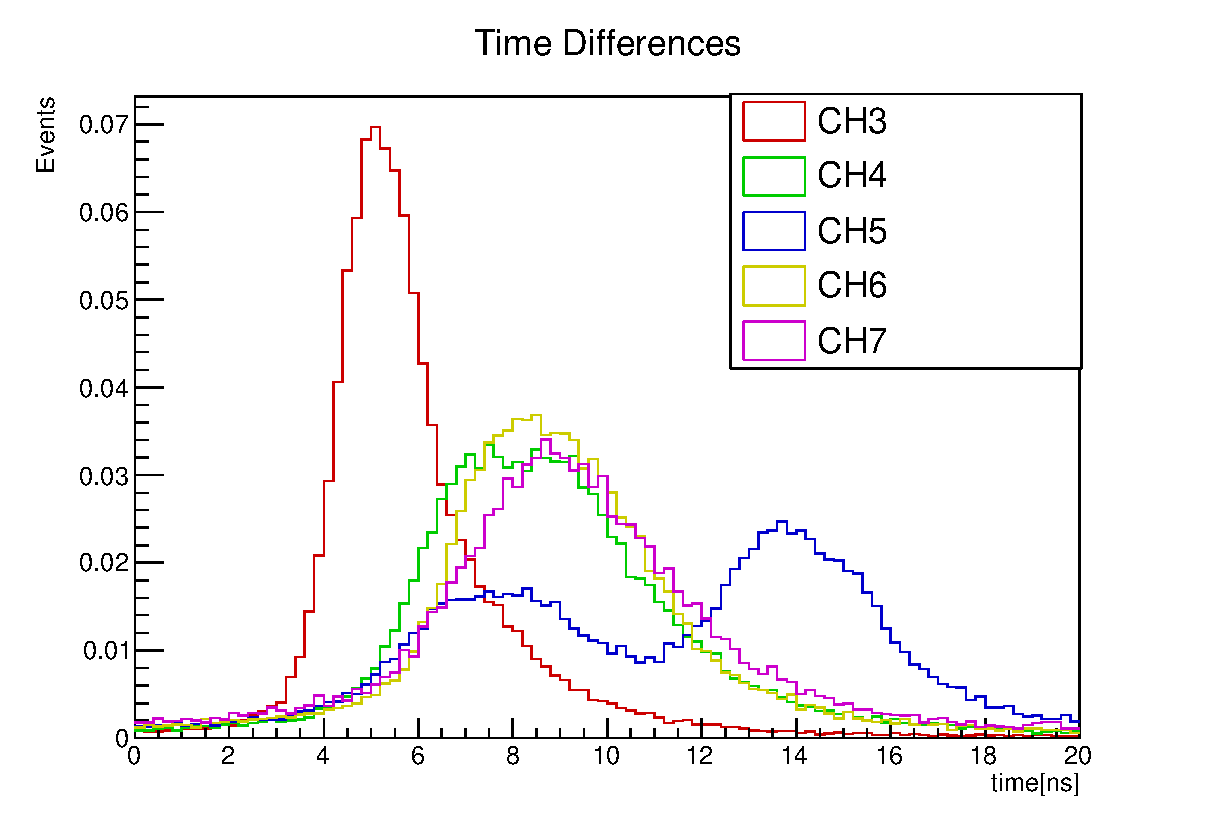
\includegraphics[width=0.8\textwidth]{figure/hatano/coincidence.eps}
  \caption{フィンガーカウンターと各NaIの時間差}
  \label{hatano_fig:coincidence}
\end{figure}

  %%%%%%%%ここから三野の続き%%%%%%

\subsection{NaIを用いた寿命と$g$因子の解析}
\subsubsection{使用データ}
NaIでは実験で得られたデータのうち,寿命測定用に磁場なしのデータとしてRUN15,$g$因子測定用に磁場ありのデータとしてRUN18,RUN19のデータを用いて解析を行った.
RUN15のsample数は1030点でビームが到達してから4120 (ns) ,RUN18とRUN19のsample数は2050点で8200 (ns) の時間までのデータを記録した.
解析に用いたRUNは表\ref{tab:RUN_info}のようなデータであった.

\begin{table}[H]%RUN Information
  \caption{用いたRUNの情報}
  \centering
  \begin{tabular}{cccc}\toprule
    & $B$ & Time\;(min) & Event数\\ \midrule
    RUN15 & --- & 47 & 71532 \\
    RUN18 & 56.06 & 75 & 113584 \\
    RUN19 & 53.97 & 297 & 446578 \\ \bottomrule
  \end{tabular}
  \label{tab:RUN_info}
\end{table}

以下の図\ref{fig:no_mag}-\ref{fig:with_mag_RUN19}は解析に用いた磁場なしと磁場ありの場合の時間分布で中心のNaIとfinger counterでコインシデンスを取った.
% コインシデンスという表現でいいか?
\begin{figure}[H]
  \centering
  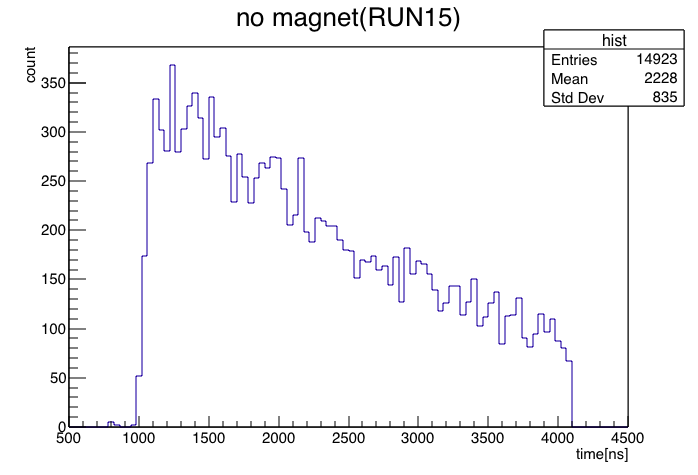
\includegraphics[width  = 0.5\textwidth]{figure/mino/no_mag.png}
  \caption{磁場がないときの時間分布(RUN15)}
  \label{fig:no_mag}
  \begin{minipage}{0.45\hsize}
    \centering
    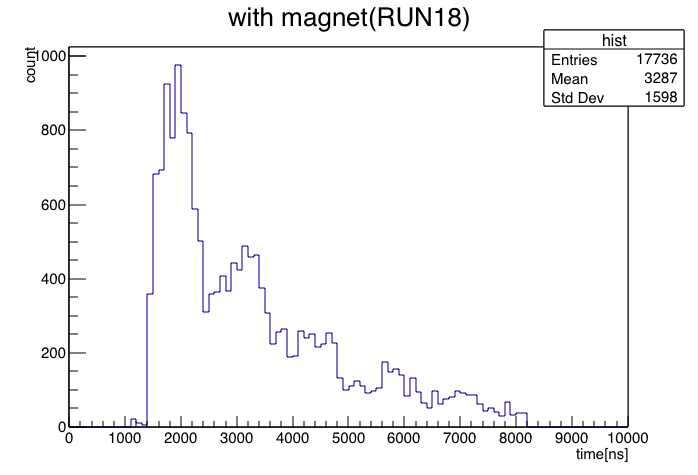
\includegraphics[width  = 1.0\textwidth]{figure/mino/with_mag_RUN18.png}
    \caption{磁場があるときの時間分布(RUN18)}
  \end{minipage}
  \begin{minipage}{0.45\hsize}
    \centering
    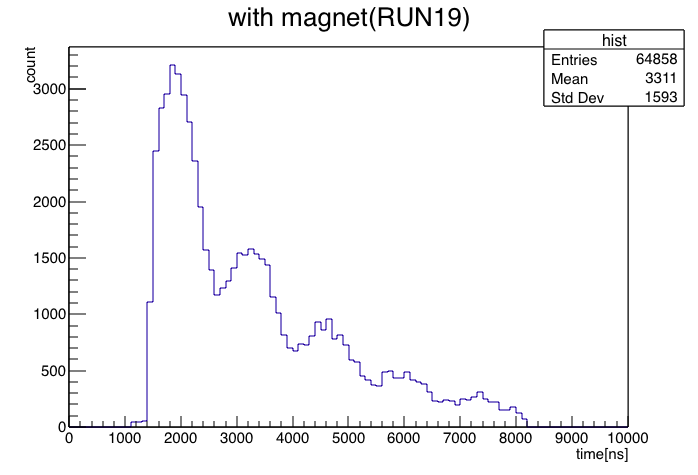
\includegraphics[width  = 1.0\textwidth]{figure/mino/with_mag_RUN19.png}
    \caption{磁場があるときの時間分布(RUN19)}
    \label{fig:with_mag_RUN19}
  \end{minipage}
\end{figure}

%--------- peak ratio -----------------------------------------------------------

\subsubsection{時間分解能}
ピークに対する一定の高さの比(50\%)を超えたところを信号の時間として用いて寿命と$g$因子のフィッティング
を行った.
以下の図\ref{fig:Original}は中心のNaIとフィンガーカウンターでコインシデンスを取った時の図で, 縦軸が時間差,横軸が中心のNaIで落としたエネルギーを表していて,この図からエネルギーに対して時間差がほとんど一定でTQ補正の必要はないことが確認できる.

\begin{figure}[H]%TQ compensation check
  \centering
  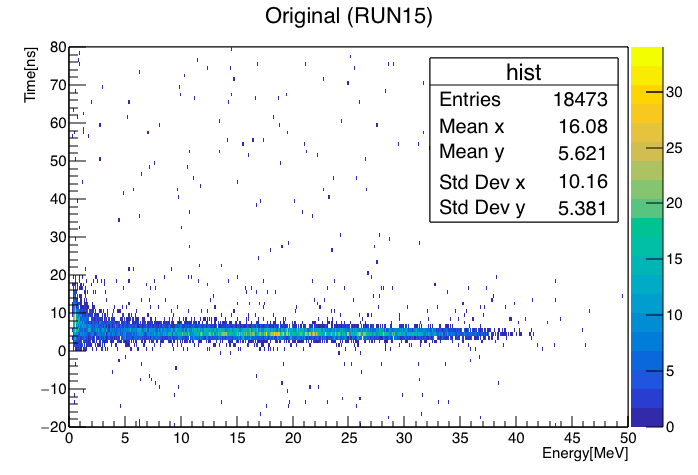
\includegraphics[width  = 0.5\textwidth]{figure/mino/Original.png}
  \caption{中心のNaIとフィンガーカウンターの時間差}
  \label{fig:Original}
\end{figure}

ただし,時間分解能が低エネルギーでは波形信号が小さい影響で高エネルギー側と比べて悪いため,5MeVより高いエネルギーの信号を用いて解析を行った.
以下の図\ref{fig:NaI_peak_gaus_fitting}は1MeV毎にエネルギーで区切って時間を
gaussianでフィッティングし,図\ref{fig:NaI_peak_time_resolution}はフィッティングで得た
時間分解能$\sigma$を横軸をエネルギーとしてプロットしたもので低エネルギーは時間分解能が悪いことが確認できる.

\begin{figure}[H]%time resolution
  \begin{minipage}{0.5\hsize}
    \centering
    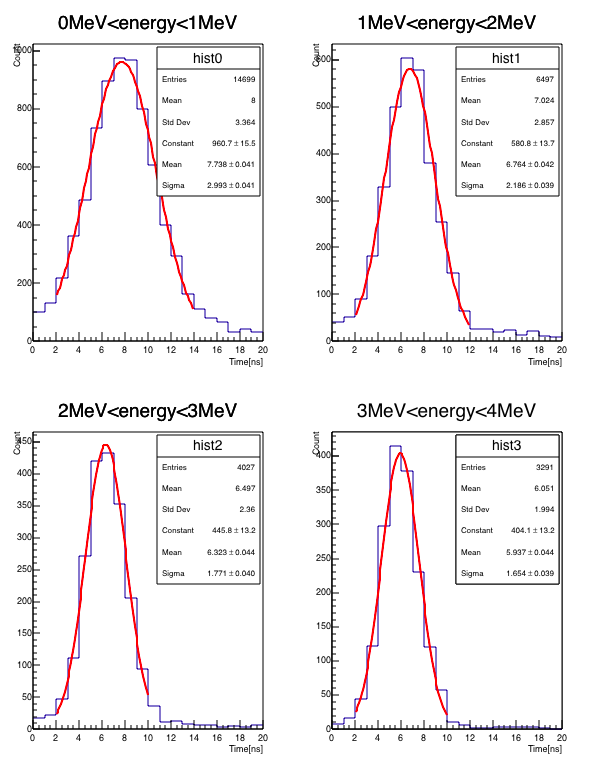
\includegraphics[width  = 0.8\textwidth]{figure/mino/gausfitting_ratio.png}
    \caption{gaussianのfitting}
    \label{fig:NaI_peak_gaus_fitting}
  \end{minipage}
  \begin{minipage}{0.5\hsize}
    \centering
    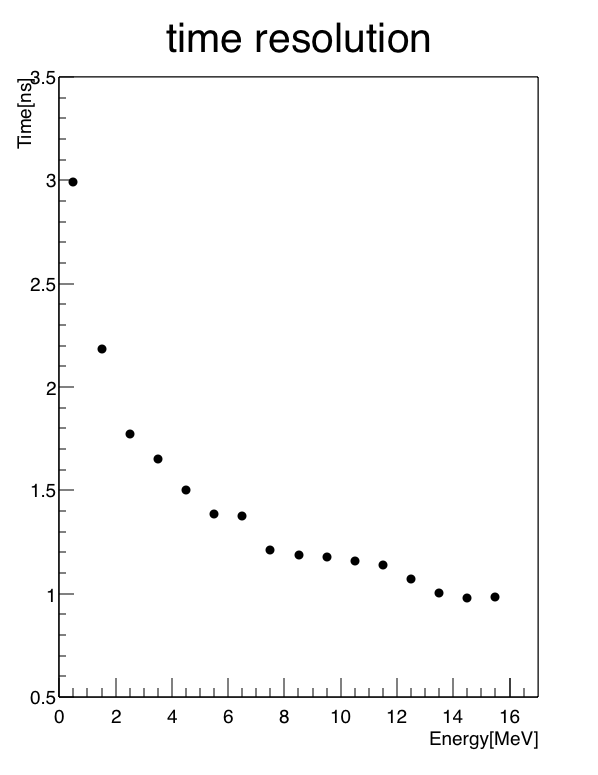
\includegraphics[width  = 0.8\textwidth]{figure/mino/timeresolution_ratio.png}
    \caption{1MeV毎に時間分解能をプロット}
    \label{fig:NaI_peak_time_resolution}
  \end{minipage}
\end{figure}

%-------- lifetime fitting ----------------------------------------------------------

\subsubsection{ミューオン寿命解析}

銅板標的を用いたRUN15の解析からミューオンの寿命を求めた.
得られた時間分布に対して以下の式(\ref{eq:lifetime})で表される寿命の関数$f(t)$を用いてフィッティングを行った.
プラスチックシンチレータの場合と同様にバックグラウンドの影響を加味して定数項を加え,RUN15のデータは4120 (ns) までしかデータを記録していなかったため,フィッティング範囲は1200 (ns) から4000 (ns) とした.統計誤差はROOTのフィッティングによるものである.
%プラスチックシンチレータ側は定数項を含まないフィッティングもしている。
\begin{gather}
  f(t) = A\exp(-\frac{t}{\tau})+C \label{eq:lifetime}\\
  \tau = 2.184 \pm 0.052 \;\;[\mu s] \notag
\end{gather}
\begin{figure}[H]
  \centering
    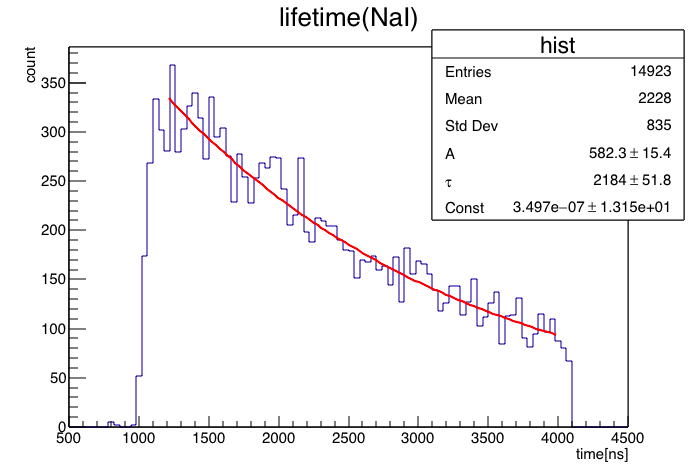
\includegraphics[width  = 0.7\textwidth]{figure/mino/lifetime_NaI_ratio.png}
    \caption{寿命フィッティング}
\end{figure}

%--------- g factor ---------------------------------------------------------------

\subsubsection{ミューオン$g$因子解析}

次に磁場標的を用いたRUN18とRUN19の解析からミュオンの$g$因子を求めた.
RUN18のデータは全Eventを用いて解析を行ったが,RUN19は先述の通り途中で磁石が外れて磁場の値が変化したため,磁場の変化を確認した結果から最初の30000 Eventsを除いたデータを用いた.
RUN18とRUN19から得られた時間分布に対して以下の式(\ref{eq:gfactor})で表される$g$因子の関数$g(t)$を用いてフィッティングを行った.
ここで寿命解析の時と同様に定数項を加え,フィッティング範囲は振動がきちんと見えている1600 ns から8000 ns までとした.
RUN18とRUN19のフィッティング結果をまとめると表\ref{tab:gfactor_result}となった.
ただし表\ref{tab:gfactor_result}において$g$因子の計算にはプラスチックシンチレータの場合と同様に各点の磁場をビームプロファイルのガウシアン加重平均した値で,RUN18では$B$=56.06 (G),RUN19では$B$=53.97 (G)という値を用いた.
また,統計誤差としてはROOTのフィッティングによって得られたものを載せており,磁場の影響を含めたものについては後述する.

\begin{gather}
  g(t) = A\exp(-\frac{t}{\tau})\{1+B\cos(\omega t+\delta)\}+C   \label{eq:gfactor}
\end{gather}
\begin{table}[H]
  \caption{フィッティングで得たRUN18とRUN19の$\omega$と$g$因子}
  \centering
  \begin{tabular}{cccc}\toprule
    & $\tau \;[\mu s]$ & $\omega \;[\;/\mu s]$ & $g$ \\ \midrule
    RUN18 & 2.010 $\pm$ 0.048 & 4.923 $\pm$ 0.024 & 2.086 $\pm$ 0.010  \\
    RUN19 & 2.126 $\pm$ 0.030 & 4.630 $\pm$ 0.015 & 2.038 $\pm$ 0.007 \\ \bottomrule
  \end{tabular}
  \label{tab:gfactor_result}
\end{table}

\begin{figure}[H]
  \begin{minipage}{0.5\hsize}
    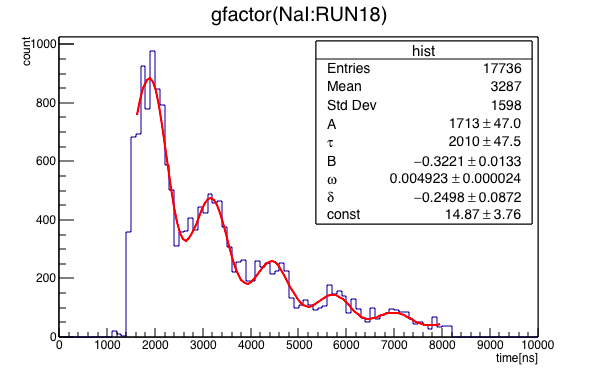
\includegraphics[width  = 1.0\textwidth]{figure/mino/gfactor_ratio_RUN18.png}
    \caption{RUN18を用いた$g$因子のフィッティング}
  \end{minipage}
  \begin{minipage}{0.5\hsize}
    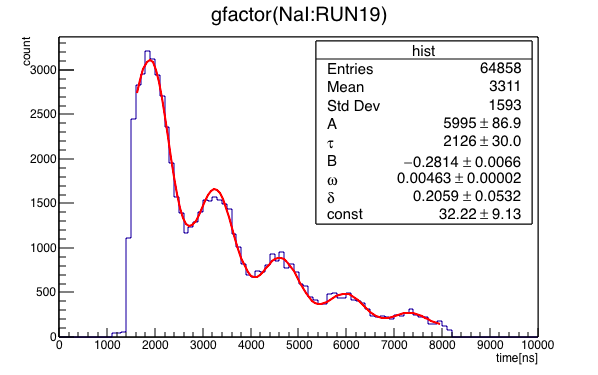
\includegraphics[width  = 1.0\textwidth]{figure/mino/gfactor_ratio_RUN19.png}
    \caption{RUN19を用いた$g$因子のフィッティング}
  \end{minipage}
\end{figure}

%-------- systematic error -------------------------------------------------------

\subsubsection{磁場の系統誤差について}

プラスチックシンチレータの場合と同様にRUN18とRUN19の$g$因子解析に用いた磁場の値はビームプロファイルをもとに加重平均をとった値であるため,ビームの不定性による磁場の
加重平均の誤差を考察した.\\
ビーム強度のガウシアンの広がり$\sigma_{x},\sigma_{y}$を動かしてRUN18とRUN19の場合での加重平均磁場の最大値と最小値を求めたところ表\ref{tab:mag_max_min}のようになった.

\begin{table}[H]
  \caption{$\sigma_{x},\sigma_{y}$を動かした時の最大磁場と最小磁場}
  \centering
  \begin{tabular}{ccc}\toprule%最大磁場と最低磁場
         & $B_{max}$ &  $B_{min}$   \\ \midrule
    RUN18 & 56.58\;($\sigma_{x}=3.3,\sigma_{y}=1.0$) & 55.82\;($\sigma_{x}=3.9,\sigma_{y}=2.9$)  \\
         RUN19 & 54.44\;($\sigma_{x}=3.9,\sigma_{y}=1.0$) & 53.76\;($\sigma_{x}=3.9,\sigma_{y}=1.0$) \\ \bottomrule
  \end{tabular}
  \label{tab:mag_max_min}
\end{table}

磁場が最大・最小,そしてビームプロファイルのときの$g$因子を求めると以下の表\ref{tab:mag_g}の値が得られた.
また,磁場の測定誤差を含んだ$g$因子の統計誤差については,磁場の誤差$\delta B$
を考慮するとプラスチックシンチレータで求めた誤差伝播の式\ref{eq:PSgosa}より,$g$因子の誤差$\sigma_{B}$は以下の表\ref{tab:g_error}の値が得られた.

\begin{table}[H]
  \caption{磁場$B$の値とそれらに対応する$g$因子の値}
  \centering
  \begin{tabular}{cccc}\toprule%最大磁場と最低磁場
    & $B_{max}$ & $B$ & $B_{min}$  \\ \midrule
    RUN18 & 2.066 & 2.086 & 2.095 \\
    RUN19 & 2.020 & 2.038 & 2.046 \\ \bottomrule
  \end{tabular}
  \label{tab:mag_g}
\end{table}

\begin{table}[H]%g因子の系統誤差(磁場)
  \caption{磁場による$g$因子の誤差の伝播}
  \centering
    \begin{tabular}{ccc}\toprule
      & $\delta B$ &  $\sigma_{B}$  \\ \midrule
      RUN18 & 1.20 & 0.046  \\
      RUN19 & 2.36 & 0.089 \\ \bottomrule
    \end{tabular}
    \label{tab:g_error}
\end{table}

以上の統計誤差と系統誤差をまとめると,RUN18とRUN19の$g$因子は以下の表のようになった.
ここで誤差の第一項は磁場の影響を含めた統計誤差であり,第二項はビームプロファイルの不定性による系統誤差である.

\begin{table}[H]%g因子の誤差のまとめ
  \caption{$g$因子の誤差のまとめ}
  \centering
  \begingroup
  \renewcommand{\arraystretch}{1.2}%行間を変更
  \begin{tabular}{cc}\toprule
    &   $g$  \\ \midrule
    RUN18 & $2.086 \pm 0.046^{+0.009}_{-0.020} $  \\
    RUN19 & $2.038 \pm 0.089^{+0.008}_{-0.018} $  \\ \bottomrule
  \end{tabular}
  \endgroup
\end{table}

%\end{document}
